\documentclass[10pt,aps,pre,onecolumn,notitlepage,nofootinbib]{revtex4-2}
\usepackage{amsmath,amssymb,mathtools,bm}
\usepackage{booktabs,array,graphicx,hyperref,microtype}
\hypersetup{hidelinks}
\newcommand{\vk}{\bm k}
\newcommand{\ve}{\bm e}
\newcommand{\vu}{\bm u}
\newcommand{\vf}{\bm f}
\newcommand{\vF}{\bm F}
\newcommand{\vR}{\bm R}
\newcommand{\veta}{\bm\eta}
\newcommand{\vchi}{\bm\chi}
\newcommand{\qT}{\mathrm{qT}}
\newcommand{\qL}{\mathrm{qL}}
\newcommand{\ImH}{\operatorname{Im}_{\!H}}
\newcommand{\order}{\mathcal O}
\newcommand{\Tr}{\operatorname{Tr}}
\ifdefined\pdftrailerid\pdftrailerid{}\fi
\renewcommand{\thesection}{SM\arabic{section}}
\begin{document}
\title{Supplementary Material for: Generation of Three-Dimensional Quasi-Transverse Elastic Waves from a One-Dimensional Longitudinal Channel in a Harmonic Lattice}
\author{M. Fernandes}
\affiliation{Independent Researcher}
% Before submission, synchronize the preferred publication name and
% corresponding-author email with the main paper. ORCID: 0009-0005-3339-8793.
\date{\today}
\maketitle

This supplement records the analytic regressions, singular-integration definitions, deterministic convergence checks, scalar-model robustness data, and coefficient-blind real-time controls used by the main text. Machine-readable records and producer code are provided in the validation archive described in the main paper's Data Availability Statement. Large real-space snapshot arrays are regenerated using the documented validation workflow rather than distributed in the compact archive. No result described here upgrades the discrete-lattice finite-coupling-region claim to a continuum, polarization-control, gauge, or electromagnetic theory.

Where the finite reference device is indexed locally, $s=1,\ldots,N_c$ denotes global active segment $i_0+s-1$, $g_s\equiv g_{i_0+s-1}$, and segment $s$ joins local line sites $q_{s-1}$ and $q_s$.

\section{Harmonic expansion, force identities, and finite source}

For a bond family $\alpha$ with equilibrium vector $\bm d=r_{0,\alpha}\hat{\bm d}$, assume $V_\alpha\in C^3$ locally,
\begin{equation}
 V_\alpha'(r_{0,\alpha})=0,
 \qquad V_\alpha''(r_{0,\alpha})=\kappa_\alpha>0.
\end{equation}
For $|\Delta\vu|\ll r_{0,\alpha}$,
\begin{align}
 |\bm d+\Delta\vu|-r_{0,\alpha}
 &=\hat{\bm d}\cdot\Delta\vu
 +\frac{|\Delta\vu|^2-(\hat{\bm d}\cdot\Delta\vu)^2}{2r_{0,\alpha}}
 +\order(|\Delta\vu|^3/r_{0,\alpha}^2),\\
 V_\alpha(|\bm d+\Delta\vu|)-V_\alpha(r_{0,\alpha})
 &=\frac{\kappa_\alpha}{2}(\hat{\bm d}\cdot\Delta\vu)^2
 +\order(\Lambda_\alpha|\Delta\vu|^3).
\end{align}
The production model is the exact quadratic Hamiltonian defined by the retained term.  The line, axial-bulk, face-diagonal, and source-link rest lengths are $a$, $a$, $\sqrt2a$, and $\sqrt3a/2$, respectively.

For one source corner $c=(s_y,s_z)$, define
\begin{equation}
 A_{ic}=u_{ic,x}-\bar q_i,
 \qquad
 B_{ic}=s_yu_{ic,y}+s_zu_{ic,z}+\frac{\Delta q_i}{2}.
\end{equation}
The two physical signed extensions obey
\begin{equation}
 e_L=\frac{A_{ic}+B_{ic}}{\sqrt3},
 \qquad
 e_R=\frac{B_{ic}-A_{ic}}{\sqrt3},
\end{equation}
so that
\begin{equation}
 \frac{g_i}{2}(e_L^2+e_R^2)=\frac{g_i}{3}(A_{ic}^2+B_{ic}^2),
 \quad
 H_{X,ic}=\frac{g_i}{4}(e_L-e_R)^2,
 \quad
 H_{R,ic}=\frac{g_i}{4}(e_L+e_R)^2.
\end{equation}
The complete coupling sectors are
\begin{equation}
 H_X=\sum_{i\in\mathcal I_c}\sum_{s_y,s_z=\pm1}H_{X,ic},
 \qquad
 H_R=\sum_{i\in\mathcal I_c}\sum_{s_y,s_z=\pm1}H_{R,ic},
 \qquad H_c=H_X+H_R.
\end{equation}
Symbolic differentiation reproduces all three corner-force components and both scalar endpoint generalized forces exactly. A randomized five-point force-gradient test gives maximum scaled error $4.21\times10^{-14}$.

For any declared finite truncation, collect the signed longitudinal bond extensions in a compatibility matrix $\mathsf B_{\rm comp}$ and the positive spring constants in a diagonal matrix $W$. Then
\begin{equation}
 K=\mathsf B_{\rm comp}^{\mathsf T}W\mathsf B_{\rm comp},
 \qquad
 \ker K=\ker\mathsf B_{\rm comp},
\end{equation}
which makes nonnegativity and exact extension-preserving zero modes explicit. Here the distinct symbol $\mathsf B_{\rm comp}$ avoids confusion with the local source coordinate $B_{ic}$.

Under the declared free-boundary and included-bond convention, representative bulk boxes of sizes $2\times2\times2$, $3\times2\times2$, $3\times3\times3$, and $4\times3\times3$ each have six rigid-body modes---three translations and three rotations. One- through four-segment combined line--bulk fixtures each have nullity two. If the finite bulk framework is infinitesimally rigid, the scalar line is connected, and at least one complete positive four-corner/eight-link source motif is present, the exact combined kernel is spanned by common axial translation and rigid bulk rotation about the line. Removing the source coupling restores the seven disconnected rigid/line modes. The complete coordinate ordering, included-bond convention, singular-value tolerance, fixture results, and mutation controls are provided in the validation archive.

The line-driven radial source is
\begin{equation}
 \vf^{\rm src}_{R,ic}=-\frac{g_i}{3}\Delta q_i(s_y\hat{\bm y}+s_z\hat{\bm z}).
\end{equation}
For the four corners,
\begin{equation}
 \sum_c\vf^{\rm src}_{R,ic}=0,
 \qquad
 \sum_c\bm r_c\times\vf^{\rm src}_{R,ic}=0,
 \qquad
 M^R=-\frac{2g_i a\Delta q_i}{3}\operatorname{diag}(0,1,1).
\end{equation}
The dipole is contractile for extension and extensile for compression.  The complete force/torque closure is restricted to the centered $C_{4v}/A_1$ sector; an off-symmetry negative control gives nonzero transverse endpoint reactions.

For an arbitrary fixed-frequency dressed line state, write
\begin{equation}
 q_i(\tau)=\operatorname{Re}[Q_i^{\rm full}(\omega)e^{-i\omega\tau}],
 \qquad
 \bar Q_i^{\rm full}=\frac{Q_i^{\rm full}+Q_{i+1}^{\rm full}}{2},
 \qquad
 \Delta Q_i^{\rm full}=Q_{i+1}^{\rm full}-Q_i^{\rm full}.
\end{equation}
The full finite-slab radial-source transform is
\begin{align}
 \widetilde{\vf}^{\rm slab}_{R}(\vk;\omega)
 &=\frac{4i}{3}\bm s_\perp(\vk)
 \sum_{i\in\mathcal I_c}g_i\Delta Q_i^{\rm full}(\omega)
 e^{-ik_x(i+1/2)a},\\
 \bm s_\perp(\vk)&=
 \begin{pmatrix}
 0\\ \sin(k_ya/2)\cos(k_za/2)\\
 \cos(k_ya/2)\sin(k_za/2)
 \end{pmatrix}.
\end{align}
The axial-average source component is
\begin{equation}
 \widetilde{\vf}^{\rm slab}_{X}(\vk;\omega)
 =\frac{8}{3}\hat{\bm x}
 \cos(k_ya/2)\cos(k_za/2)
 \sum_{i\in\mathcal I_c}g_i\bar Q_i^{\rm full}(\omega)
 e^{-ik_x(i+1/2)a},
\end{equation}
and the complete line-driven source transform is
\begin{equation}
 \widetilde{\vf}^{\rm slab}_{X+R}
 =\widetilde{\vf}^{\rm slab}_{X}
 +\widetilde{\vf}^{\rm slab}_{R}.
\end{equation}
For the special pure Bloch component $Q_i=Qe^{i\kappa ia}$, the axial part reduces to
\begin{equation}
 \widetilde{\vf}^{\rm slab}_{X}(\vk;\kappa)
 =\frac{8Q}{3}\cos(\kappa a/2)\,
 \mathcal A(\kappa-k_x)
 \cos(k_ya/2)\cos(k_za/2)\hat{\bm x},
\end{equation}
while the radial part reduces to
\begin{align}
 \widetilde{\vf}^{\rm slab}_{R}(\vk;\kappa)
 &=-\frac{8Q}{3}\sin(\kappa a/2)\,
 \mathcal A(\kappa-k_x)\bm s_\perp(\vk),\\
 \mathcal A(\kappa-k_x)
 &=\sum_{i\in\mathcal I_c}g_i e^{i(\kappa-k_x)(i+1/2)a}.
\end{align}
These pure-Bloch $X$ and $R$ components define the complete bare $X+R$ source used in the shell-overlap witnesses of SM2. A direct segment/corner sum with independently randomized $\kappa$ and $k_x$ agrees below $2\times10^{-14}$ scaled error. Because the radial-source resultant vanishes, its first moment controls the leading transverse-wave-number term,
\begin{equation}
 \widetilde{\vf}^{\rm src}_{R,i}(\vk_\perp)
 =-i\bm M_i^R\vk_\perp
 +\order(g_i|\Delta q_i|a^3|\vk_\perp|^3).
\end{equation}
Moreover,
\begin{equation}
 \|\bm s_\perp(\vk)\|^2
 =\frac{1-\cos(k_ya)\cos(k_za)}{2},
\end{equation}
Because this factor is independent of $k_x$, its exact nodal set in the closed transverse first Brillouin zone consists of the full axial line $(k_y,k_z)=(0,0)$ and the periodically identified axial lines through the transverse zone corners $(k_y,k_z)=(\pm\pi/a,\pm\pi/a)$, for every allowed $k_x$. After removing the segment-midpoint phase, the leading radial-source amplitude has order two and the post-leading remainder order four. For $k_\perp=(k_y^2+k_z^2)^{1/2}>0$, define
\begin{align}
 \ve_L&=\vk/|\vk|,\\
 \ve_{SH}&=k_\perp^{-1}(0,-k_z,k_y)^T,\\
 \ve_{SV}&=|\vk|^{-1}\left(k_\perp,-\frac{k_xk_y}{k_\perp},-\frac{k_xk_z}{k_\perp}\right)^T,
\end{align}
and let $V_\nu^p=\ve_p^\dagger\widetilde{\vf}^{\rm src}_\nu$ denote a complex source-projection amplitude, not a power. Under the common scaling $(\vk,\kappa)=\rho(\widehat\vk,\widehat\kappa)$ at fixed regular non-axial direction,
\begin{equation}
 V_X^{SV}=\order(1),
 \qquad V_R^{SV}=\order[(\rho a)^2],
 \qquad V_R^{SH}=\order[(\rho a)^4].
\end{equation}
These are source asymptotics, not finite-frequency branch definitions or contribution fractions.

\section{Bulk spectrum, shell refinement, and exact core symmetry}

For positive axial and face-diagonal stiffnesses,
\begin{equation}
 D(\vk)=\frac{2}{m_b}\sum_{\bm d}K_{\bm d}[1-\cos(\vk\cdot\bm d)]\hat{\bm d}\hat{\bm d}^{T}.
\end{equation}
The sum-of-squares argument gives three translations at $\Gamma$ and no nontrivial Bloch zero mode for $\vk\ne0$.  For $K_{\rm axis}=K_{\rm diag}=K$,
\begin{equation}
 D(\vk)=\frac{Ka^2}{m_b}(|\vk|^2I+2\vk\vk^T)+\order(Ka^4|\vk|^4/m_b),
\end{equation}
so $c_T=a\sqrt{K/m_b}$ and $c_L=\sqrt3c_T$.

Root-refined optimization on the branch shells $\Sigma_\lambda(1.2)$ gives the conservative operating-point bounds
\begin{equation}
 \min_{\Sigma_0\cup\Sigma_1\cup\Sigma_2}(\omega_2^2-\omega_1^2)>0.9390,
 \quad
 \max_{\Sigma_0\cup\Sigma_1}\hat{\vk}^{\dagger}P_{\qT}\hat{\vk}<1.25\times10^{-3},
\end{equation}
\begin{equation}
 \min_{\Sigma_2}\hat{\vk}^{\dagger}P_{\qL}\hat{\vk}>0.99988.
\end{equation}
Every extremizing point is projected back to its exact shell with squared-frequency residual below $10^{-12}$ and is checked by a second optimization parameterization. Projector tests use only projector quantities or covariantly transformed cluster operators; arbitrary $U(2)$ mixtures of distinct eigenvalues are not treated as alternative modes.

Where $\omega_2^2$ is separated from the lower pair, the upper projector can be written without choosing a lower-doublet basis,
\begin{equation}
 P_{\qL}(\vk)=
 \frac{[D(\vk)-\omega_0^2I][D(\vk)-\omega_1^2I]}
 {(\omega_2^2-\omega_0^2)(\omega_2^2-\omega_1^2)},
 \qquad P_{\qT}=I-P_{\qL}.
\end{equation}
This remains well defined at an internal degeneracy of the lower pair, provided the upper/lower gap remains nonzero.

\begin{table}[htbp]
\caption{Regular lower-shell source-overlap witnesses at $\omega=1.2$. The source is the complete bare finite-slab $X+R$ line-driven source; the radial-component overlap is shown separately. Here $\bm v_g=\nabla_{\bm k}\omega_\lambda$. The listed $\bm k a$ values are rounded for display; shell residuals, group speeds, gaps, and overlaps are evaluated at the corresponding full-precision machine-readable coordinates. Group speeds are in units of $a\sqrt{K_{\rm diag}/m_b}$. The raw squared-overlap columns use $Q/a=1$ (hence $Q=1$ at the reference $a=1$) and scale as $|Q|^2$.}
\begin{ruledtabular}
\begin{tabular}{c c c c c c}
branch & $\bm k a$ & $|\omega_\lambda^2-1.44|$ & $|\bm v_g|$ & $|\bm e_\lambda^\dagger\widetilde{\bm F}_{X+R}|^2$ & $|\bm e_\lambda^\dagger\widetilde{\bm F}_{R}|^2$\\
\hline
0 & $(1.022121,\ 0.711990,\ -0.020432)$ & $<10^{-12}$ & $0.894276$ & $1.151778$ & $0.0593474$\\
1 & $(0.880718,\ 0.217031,\ -0.851447)$ & $<10^{-12}$ & $0.895775$ & $3.495846$ & $0.132790$\\
\end{tabular}
\end{ruledtabular}
\end{table}
The lower-branch splits at these points are $0.00596289$ and $0.01596669$, and the upper gaps are $2.41843$ and $2.41369$, respectively. Only strict nonzero overlap is used in the existence argument; these raw magnitudes are not transmission coefficients.

Let $B=(|X_1\rangle,|R_1\rangle,\ldots,|X_6\rangle,|R_6\rangle)$, let $V_c\in\mathbb R^{72\times7}$ be the full line-to-core map, and let $U_c\in\mathbb R^{72\times72}$ be the full local source-link stiffness on the core.  The exact finite-core statements are
\begin{equation}
 B^{\dagger}B=I_{12},
 \quad P_{A_1}^{(c)}=BB^{\dagger},
 \quad P_{A_1}^{(c)}V_c=V_c,
 \quad [P_{A_1}^{(c)},U_c]=0,
 \quad [P_{A_1}^{(c)},G_{cc}^R]=0.
\end{equation}
The reduced matrices used below are $V=B^\dagger V_c$ and $U=B^\dagger U_cB$. The full bulk stiffness preserves the infinite-dimensional $A_1$ sector but not the finite spatial support of the source core. The exact $72\to12$ reduction applies after the exterior bulk is retained through the projected resolvent. With $P=P_{A_1}^{(c)}=BB^\dagger$ and Frobenius norm $\|\cdot\|_F$, define
\begin{align}
 \epsilon_V&=\frac{\|(I-P)V_c\|_F}{\|V_c\|_F},
 &\epsilon_U&=\frac{\|(I-P)U_cB\|_F}{\|U_cB\|_F},\\
 \epsilon_G&=\frac{\|(I-P)G_{cc}^RB\|_F}{\|G_{cc}^RB\|_F},
 &\epsilon_{[G,P]}&=\frac{\|G_{cc}^RP-PG_{cc}^R\|_F}{\|G_{cc}^R\|_F}.
\end{align}
The archived regression uses $(\omega,\eta,N)=(1.2,0.03,32)$ and also compares the full and reduced core fields and effective self-energies. All source, stiffness, projected-resolvent, commutator, field, and self-energy residuals lie between $10^{-16}$ and approximately $2\times10^{-15}$. The analytic symmetry proof, rather than this finite-grid regression, is the controlling reason the reduction is exact.

\section{Retarded response, physical flux normalization, and local current}

Distinguish the infinite bulk, its 72-coordinate core projection, and the centered reduction. Here $K_b$ is the Hessian of $H_b$ and $M_b=m_bI$ on the bulk displacement space:
\begin{equation}
 \mathcal G_b^R=[K_b-(\omega+i0^+)^2M_b]^{-1},
 \quad G_{cc,0}^R=E_c^{\dagger}\mathcal G_b^R E_c,
 \quad g_0^R=B^{\dagger}G_{cc,0}^RB.
\end{equation}
For finite-core form factor
\begin{equation}
 [\bm\Phi_\lambda(\vk)]_A
 =\sum_{r\mu\in c}B_{r\mu,A}^*e_{\lambda\mu}(\vk)e^{i\vk\cdot\vR_r},
\end{equation}
use
\begin{align}
 g_0^R(\omega)
 &=\frac{a^3}{(2\pi)^3m_b}\sum_\lambda\int_{\rm BZ}
 \frac{\bm\Phi_\lambda\bm\Phi_\lambda^{\dagger}}
 {\omega_\lambda^2-(\omega+i0^+)^2}\,d^3k,\\
 \ImH g_{0,C}^R
 &=\frac{\pi a^3}{(2\pi)^3m_b}\int_{\rm BZ}\sum_{\lambda\in C}
 \bm\Phi_\lambda\bm\Phi_\lambda^{\dagger}
 \delta(\omega_\lambda^2-\omega^2)\,d^3k\succeq0.
\end{align}
The co-area form is used only on regular patches.  The modal lower cluster is $C=\{0,1\}$; the wave-normal geometric matrix is a separate diagnostic.

The dressed reduced core and bulk self-energy are
\begin{equation}
 g_c^R=(I+g_0^RU)^{-1}g_0^R,
 \qquad
 \Sigma_b^R=-V^{\dagger}g_c^RV.
\end{equation}
For one scalar channel in each lead,
\begin{equation}
 \sigma_q^R=-K_qe^{i\kappa a},
 \qquad \gamma_q=2K_q\sin(\kappa a).
\end{equation}
The Caroli-normalized device response and effective source are
\begin{equation}
 \vchi_D^{(L)}=G_D^R\Gamma_L^{1/2}|L\rangle,
 \qquad
 \veta_c=(I+Ug_0^R)^{-1}V\vchi_D^{(L)}.
\end{equation}
Under the real-field convention $x(\tau)=\operatorname{Re}[Xe^{-i\omega\tau}]$, the physical unit-energy-flux response is $2\vchi_D^{(L)}/\sqrt\omega$ and the physical effective force is $-2\veta_c/\sqrt\omega$.  For an arbitrary physical core force $\vf$ and displacement $\vu=g_0^R\vf$, the corresponding work identity is
\begin{equation}
 \overline P_C=\frac{\omega}{2}\vf^{\dagger}\ImH g_{0,C}^R\vf.
\end{equation}
For the physical unit-incident-flux effective force $\vf=\vf_{c,{\rm phys}}^{\rm eff}=-2\veta_c/\sqrt\omega$, this becomes $\overline P_C=T_C$. This distinguishes the effective source from the reduced core displacement $-g_0^R\veta_c$.

Assigning half of each pair energy to each endpoint gives the exact directed current
\begin{equation}
 J_{i\to j}=-\frac12(\bm v_i+\bm v_j)\cdot\bm F_{i\leftarrow j},
 \qquad
 \dot h_i+\sum_{j\sim i}J_{i\to j}=0.
\end{equation}
For a simple Bloch mode the cell-averaged current equals modal energy times group velocity.  Local coherent fields may retain cross terms; channel additivity is an asymptotic flux-bilinear or outgoing-packet statement.  At exact degeneracy, the physical channels are fixed by the complete commuting little-group operators when available; otherwise only the explicitly defined cluster observable is used.

As a device-partition regression, moving up to four pristine scalar cells independently across either lead/device boundary for both incidence directions changes all physical powers by at most $4.2\times10^{-14}$ relatively after the expected Bloch phases are removed. Define the dimensionless lead phase $\phi_\kappa=\kappa a$. If $n_{\rm inc}$ pristine cells are moved on the incident side and $n_L,n_R$ are the left/right padding counts, compare
\begin{equation}
 \vchi_{\rm active}\mapsto e^{-i\phi_\kappa n_{\rm inc}}\vchi_{\rm active},
 \quad r\mapsto e^{-2i\phi_\kappa n_{\rm inc}}r,
 \quad t\mapsto e^{-i\phi_\kappa(n_L+n_R)}t.
\end{equation} Deliberately attaching a self-energy at the wrong position changes $T_q$ by order unity, while a $1\%$ bond defect produces a resolvable response. A standalone builder with no imports from the production implementation reproduces $D(\vk)$ over 500 random wave vectors below $5.2\times10^{-16}$ scaled error and the microscopic identity $\overline{\bm{\mathcal J}}=\overline{\mathcal E}_{\lambda\bm k}\bm v_{g,\lambda}$ over 600 nondegenerate modes below $1.8\times10^{-15}$ using the analytic derivative ($2.4\times10^{-9}$ with a finite-difference velocity). An independent reconstruction of the physical paired-spring Hessian reproduces $U$, $V$, and $K_{\rm self}$ below $4.0\times10^{-16}$ relatively; direct full-block and Schur-eliminated solves agree below $1.2\times10^{-15}$ over the reference problem and 200 randomized passive finite fixtures.

A regular branch-0 weak-coupling witness at $\omega=1.2$ is
\begin{equation}
 \bm k a=(0.6318952450,-0.6028746482,-0.9641061600).
\end{equation}
The displayed coordinate is rounded; the following diagnostics are evaluated at its full-precision machine-readable counterpart. Its squared-frequency shell residual is below $10^{-12}$, $|\nabla_{\bm k}\omega_0^2|=1.8578005$, the internal lower split is $0.1007240$, the upper-cluster gap is $2.6995796$, and $|\bm\Phi_0^\dagger\veta_{c,1}|^2=0.7492079$. A $7\times7$ exact-shell neighborhood has minimum overlap $0.699897$, minimum gradient norm $1.850667$, and minimum lower/upper gaps $0.080977$ and $2.684330$, respectively. Thus the positive first-order overlap holds on a relatively open regular shell patch. These values are not finite-coupling transmission coefficients.

For normalized incident energy weights $w_j$,
\begin{equation}
 T_C^{\rm packet}=\sum_jw_jT_C(\omega_j),
 \qquad \sum_jw_j=1.
\end{equation}
The finite retained frequency interval and its outside-band energy remainder are recorded separately; the latter is a one-sided passivity bound, not a symmetric error bar.

\section{Singular integrations and reference convergence}

The controlling calculation combines an $N=192$ marching-surface co-area quadrature with an $M=256$ Jackson--Chebyshev principal-value reconstruction. The PV matrix is the equal mean of two independently scrambled Sobol samples, each with $2^{23}$ points (seeds 20260920 and 20260921), using 16384 energy bins on $[0,12]$ and Jackson margin 1.02. The same samples supply the order ladder. At degenerate grid nodes, each tied branch receives its equal-rank share of the complete projected eigenspace weight; geometric diagnostics retain the complete-cluster coherences. The validation records contain the raw matrices, basis-rotation controls and coverage diagnostics.

For sampler ensemble $r$, let $P_M^{(r)}$ be its principal-value matrix and $g_{00}^{(r)}(M)=[P_M^{(r)}]_{00}$, the $X_1$ source-sector diagonal entry. The tabulated definitions are
\begin{equation}
 \overline P_M=\frac12\sum_{r=1}^{2}P_M^{(r)},\qquad
 d_M=100\,\frac{\|\overline P_M-\overline P_{256}\|_F}{\|\overline P_{256}\|_F},\qquad
 s_{00}(M)=100\,\frac{\max_r g_{00}^{(r)}-\min_r g_{00}^{(r)}}{\frac12\sum_r g_{00}^{(r)}} .
\end{equation}
For the marching-surface matrix, $A_{\rm pre}$ denotes the raw complex assembly before reciprocal projection,
\begin{equation}
 A=\operatorname{Re}\!\left[\frac{A_{\rm pre}+A_{\rm pre}^{T}}2\right],\qquad
 \epsilon_{\rm sym}=\max\!\left[
 \frac{\|\operatorname{Im}A_{\rm pre}\|_F}{\max(\|\operatorname{Re}A_{\rm pre}\|_F,10^{-30})},
 \frac{\|A_{\rm pre}-A_{\rm pre}^{\dagger}\|_F}{\max(\|A_{\rm pre}\|_F,10^{-30})}
 \right].
\end{equation}
The listed minimum eigenvalue is evaluated after this projection. Here $\pi\rho_{\qT}^{\rm modal}=\ImH g_{0,0}^R+\ImH g_{0,1}^R$, $\pi\rho_{\qL}^{\rm modal}=\ImH g_{0,2}^R$, and $\rho_{\rm tot}=\rho_{\qT}^{\rm modal}+\rho_{\qL}^{\rm modal}$; $\epsilon_{\rm sym}$ separately measures the raw pre-projection residual. The wave-normal geometric-longitudinal matrix is retained only as a separately named diagnostic.

Table~\ref{tab:sm-physical-convergence} reports the physical six-segment ($12\times12$) kernel. The PV blocks and selected $N=192$ spectral block agree entry-for-entry with the corresponding leading blocks of the auxiliary ten-segment ($20\times20$) matrices; the spectral support-extension check was performed at this selected grid. Whole-matrix norms and eigenvalues are dimension specific.

\begin{table}[htbp]
\caption{Physical six-segment modal convergence diagnostics at $\omega=1.2$. Percentages are shown for $d_M$ and $s_{00}$; the longitudinal norm is modal branch 2, not a wave-normal geometric projection.}
\label{tab:sm-physical-convergence}
\centering\scriptsize
\setlength{\tabcolsep}{2.6pt}
\renewcommand{\arraystretch}{0.98}
\begin{ruledtabular}
\begin{tabular}{rccc@{\hspace{7pt}}rcccc}
\multicolumn{4}{c}{principal-value order ladder}&\multicolumn{5}{c}{marching-surface ladder}\\
$M$&$\|\overline P_M\|_F$&$d_M$&$s_{00}$&$N$&$\|\pi\rho_{\rm tot}\|_F$&$\|\pi\rho_{\qL}^{\rm modal}\|_F$&$\lambda_{\min}(\rho_{\rm tot})$&$\epsilon_{\rm sym}$\\
\hline
192&0.896397&0.0513\%&0.0241\%&128&1.048264&0.113662&$4.12\times10^{-8}$&$2.13\times10^{-9}$\\
256&0.896608&0.0000\%&0.0601\%&160&1.048055&0.113676&$4.06\times10^{-8}$&$3.26\times10^{-9}$\\
320&0.896530&0.0155\%&0.1774\%&192&1.047933&0.113684&$4.03\times10^{-8}$&$5.40\times10^{-10}$\\
\end{tabular}
\end{ruledtabular}
\end{table}

The independent linear-tetrahedron calculation uses an unshifted periodic grid and the six-tetrahedron $000$--$111$ body-diagonal split. It linearly interpolates the sorted eigenvalues and uses centroid spectral weights with complete-projector rank sharing at ties. The scalar retarded integral uses stable confluent divided differences with higher-precision fallbacks. Both signs of separation phase are retained when assembling the projected matrix. The choice $z=\omega^2+i10^{-10}$ selects the retarded logarithm branch rather than physical broadening. The retained generalized-Bloch corroboration extrapolates the real part from finite $\eta$.


\begin{table}[htbp]
\caption{High-resolution modal-qT sequences and generalized-Bloch extrapolations. The spans are deterministic one-factor diagnostics and are not combined into a statistical error bar.}
\begin{ruledtabular}\begin{tabular}{lcc}
category & $T_{\qT}^{\rm modal}$ values & span\\\hline
surface/PV $N=128,160,192$ & $0.12567058,\ 0.12566614,\ 0.12565926$ & $1.133\times10^{-5}$\\
tetrahedron $N=128,160,192$ & $0.12559600,\ 0.12559347,\ 0.12560796$ & $1.450\times10^{-5}$\\
GB low-pair/quadratic/linear-LS & $0.12560631,\ 0.12559580,\ 0.12562207$ & $2.6276\times10^{-5}$\\
\end{tabular}\end{ruledtabular}
\end{table}
At fixed spectral grid $N=192$, changing the mean PV order from $M=192$ to $256$ changes qT by $0.00771\%$; increasing each Sobol sample from $2^{22}$ to $2^{23}$ points at $M=256$ changes it by $0.02355\%$. An independent two-shift $160^3$ PV sample mean differs from the selected result by $0.000158\%$. Higher orders increase the scramble and shift sensitivity. These are separate observed sensitivities, not a common statistical error bar.

The three central qT estimates span $0.12560631$--$0.12565926$. Surface refinement, PV sampling/order, tetrahedron refinement and retained generalized-Bloch extrapolation remain separate numerical categories. The controlling raw flux-closure residual is $1.30\times10^{-11}$.


For the separately dressed surrogate family, define $H_c(\alpha)=H_X+\alpha H_R$ and the complete Hamiltonian $H(\alpha)=H_q+H_b+H_c(\alpha)$. Thus $\alpha$ multiplies the complete positive radial part of the coupling sector, including its core stiffness, line--core coupling, and line self-stiffness, while $H_q$ and $H_b$ remain fixed. Each point is therefore a new dressed complete solve. The 21-point sampled qT trend is shown in Fig.~\ref{fig:sm-alpha}; it is not an analytic monotonicity theorem.
\begin{figure}[htbp]
\centering
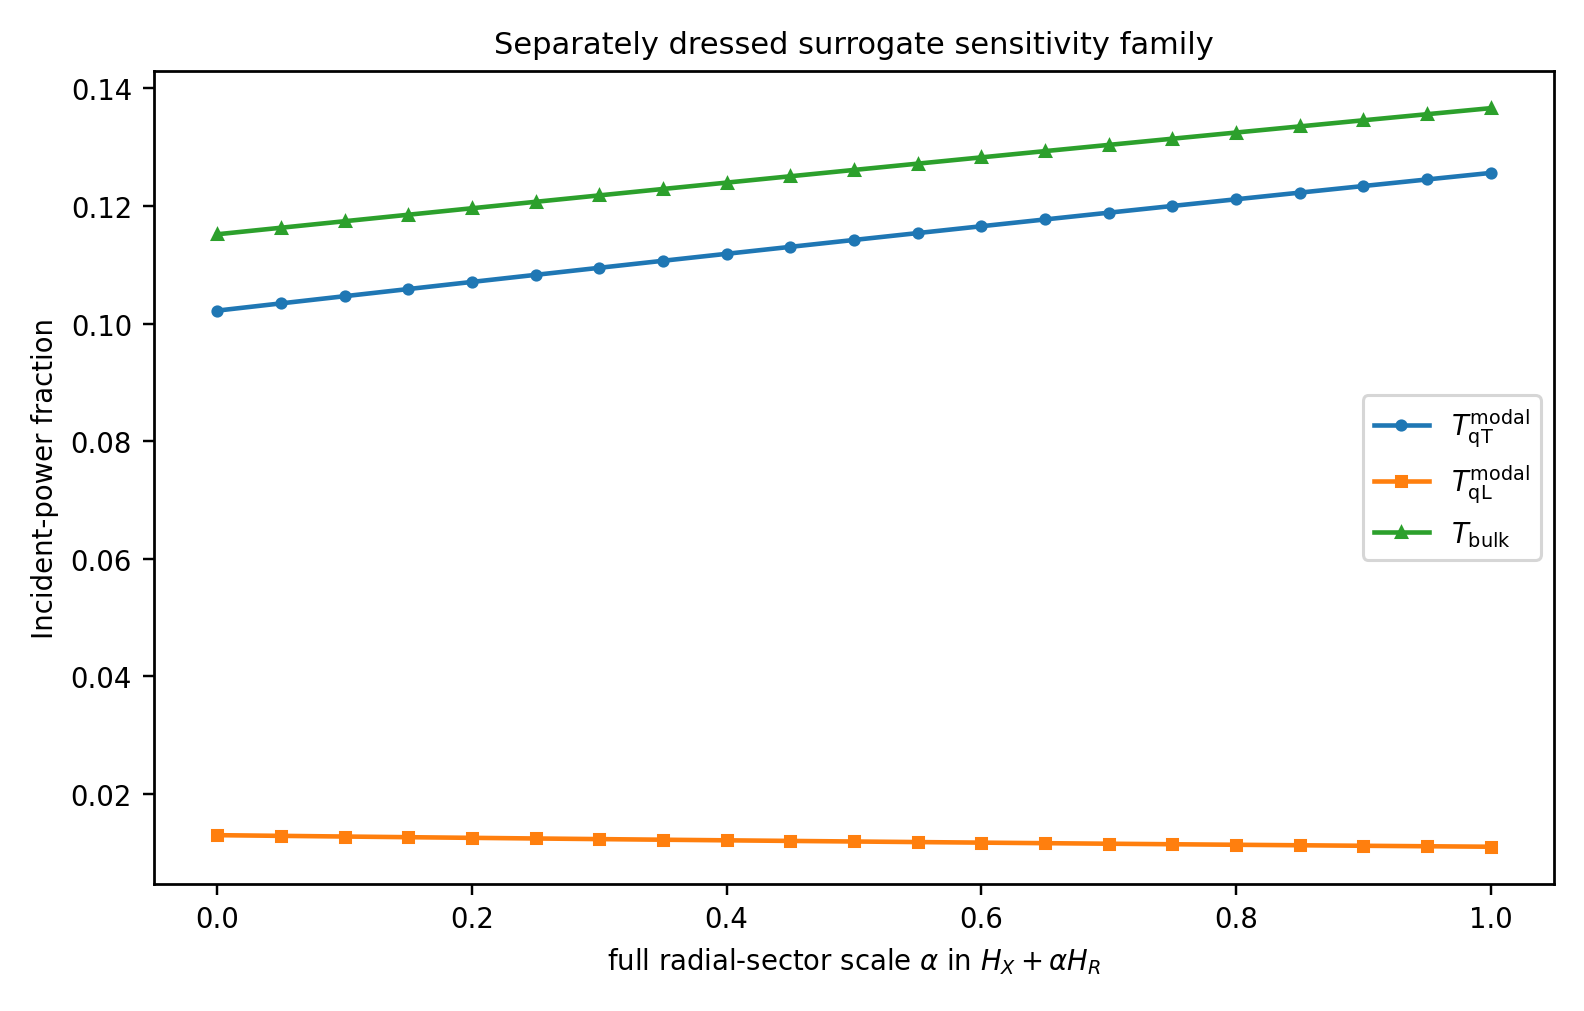
\includegraphics[width=0.72\linewidth]{figures/Halpha_transmission_scan_p06.png}
\caption{Separately dressed $H(\alpha)$ surrogate family at the reference frequency.}
\label{fig:sm-alpha}
\end{figure}
For the physical full state, decompose $V=V_X+V_R$ and set $\veta_\nu=(I+Ug_0^R)^{-1}V_\nu\vchi_D^{(L)}$ for $\nu\in\{X,R\}$, so that $\veta=\veta_X+\veta_R$. With $Q_{\qT}=\ImH g_{0,\qT}^R$, define $T_{\nu\nu}=2\veta_\nu^\dagger Q_{\qT}\veta_\nu$ and $T_{XR}=4\operatorname{Re}(\veta_X^\dagger Q_{\qT}\veta_R)$. The common-dressing decomposition obeys
\begin{equation}
 T_{\qT}^{\rm modal}=T_{XX}+T_{RR}+T_{XR}.
\end{equation}
At the controlling surface/PV point,
\begin{equation}
 (T_{XX},T_{RR},T_{XR})
 \simeq(0.10147813,0.00179177,0.02238935).
\end{equation}
The independent $N=192$ tetrahedron cross term differs by $0.026\%$. These are terms in one quadratic form, not separately conserved energies or the separately dressed ablation rows.
\begin{figure}[htbp]
\centering
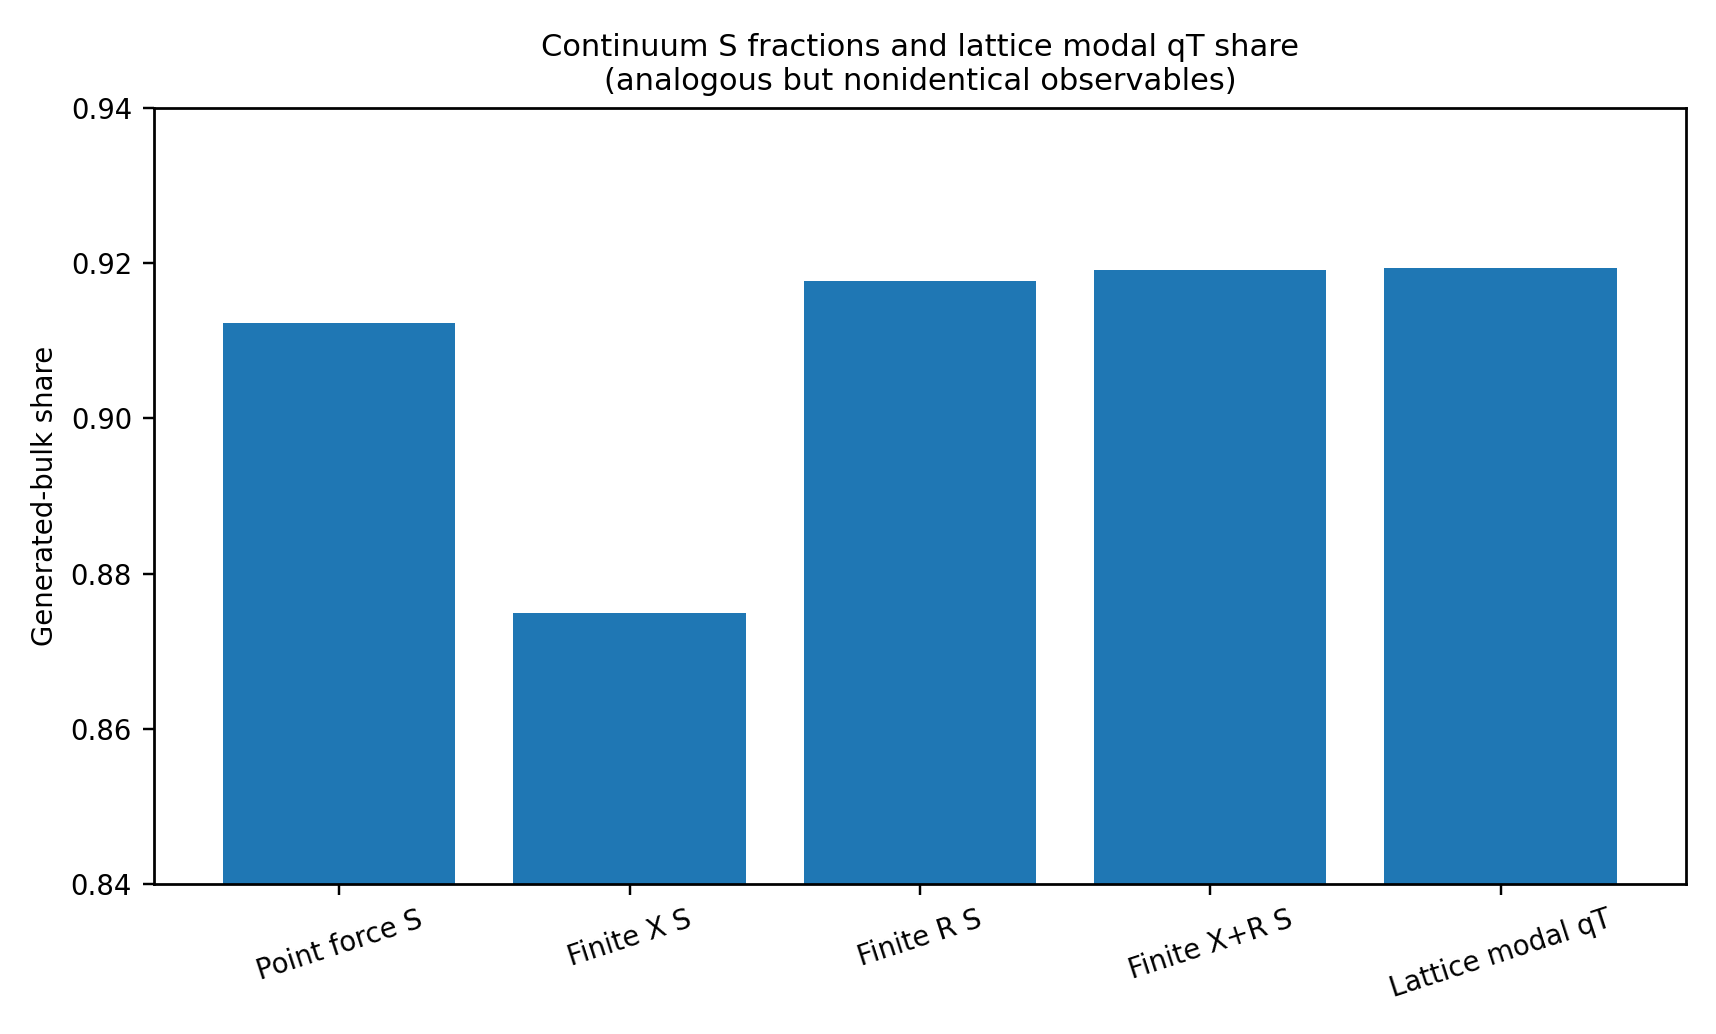
\includegraphics[width=0.72\linewidth]{figures/continuum_lattice_share_comparison_p06.png}
\caption{Continuum shear fractions and the lattice modal-qT generated-bulk share. These are analogous but nonidentical observables and the comparison does not derive the absolute lattice transmission.}
\label{fig:sm-continuum}
\end{figure}

\section{Branch-resolved modal robustness and scalar real-time controls}

\subsection{Finite parameter families}

The branch-resolved robustness calculations use
\begin{equation}
 \ImH g_{0,\qT}^R=\ImH g_{0,0}^R+\ImH g_{0,1}^R,
 \qquad
 \ImH g_{0,\qL}^R=\ImH g_{0,2}^R.
\end{equation}
Table~\ref{tab:sm-modal-robust} gives the exact finite one-factor inputs; positivity on these grids is not a theorem over a continuous interval.

\begin{table}[!htbp]
\caption{Exact branch-resolved modal-qT robustness inputs; ranges refer only to the finite tested values.}
\label{tab:sm-modal-robust}
\centering\scriptsize\setlength{\tabcolsep}{2.8pt}\renewcommand{\arraystretch}{0.96}
\begin{tabular}{@{}llccc@{}}\toprule
family&exact tested values&count&method&qT range\\\midrule
frequency&$\omega=0.600+0.025j$, $j=0,\ldots,48$&49&M2&0.10486--0.21774\\
coupling&$s=(0.05,0.075,0.10,0.15,0.20,0.25,0.50,1.00,1.50,2.00)$&10&M1&0.000246--0.52218\\
slab length&$N_c=(2,3,4,6,8,10)$; rule below&6&M1&0.00882--0.24512\\
profile&five six-segment vectors below&5&M1&0.06495--0.15787\\
line speed&$c_q=(0.65,0.8,0.9,1.0,1.1,1.2,1.3,1.5,1.7,2.0)$&10&M1&0.02646--0.12569\\
stiffness&$K_{\rm diag}/K_{\rm axis}=(0.75,0.9,1.0,1.1,1.25)$&5&M3&0.09815--0.16902\\\bottomrule
\end{tabular}

\parbox{0.99\linewidth}{\scriptsize Except where varied, $a=m_q=m_b=K_{\rm axis}=K_{\rm diag}=1$, $K_q=1.69$ ($c_q=1.3$), $\omega=1.2$, $N_c=6$, and $\bm g_{\rm ref}=(0.10,0.20,0.20,0.20,0.20,0.10)$ are fixed. M1, M2, and M3 use (PV order, surface grid) $(256,80)$, $(256,80)$, and $(160,80)$. The common medium uses the two $2^{23}$-point Sobol samples above. Each stiffness case uses its own two shifted $64^3$ grids and $2^{19}$-point Sobol sample with 6144 bins on the full spectral support $[0,(4K_{\rm axis}+8K_{\rm diag})/m_b]$; exact shifts and seeds are recorded in the archive. For $N_c=2$, $\bm g=(0.10,0.10)$; otherwise endpoints are 0.10 and interiors 0.20. Other profiles are $\bm g_{\rm uniform}=(0.20,0.20,0.20,0.20,0.20,0.20)$, $\bm g_{\rm soft}=(0.05,0.12,0.20,0.20,0.12,0.05)$, $\bm g_{\rm short}=(0,0.10,0.20,0.20,0.10,0)$, and $\bm g_{\rm edge}=(0.20,0.10,0.10,0.10,0.10,0.20)$. In the coupling family $s$ scales the reference profile and $s=0$ is a separate exact null. In the speed family $a=m_q=1$ and $K_q=c_q^2$; in the stiffness family $K_{\rm axis}=1$ is fixed while $K_{\rm diag}$ varies. Complete row-level values, numerical encodings, and producer inputs are provided in the validation archive.}
\end{table}

All 85 sampled positive-coupling qT values are positive; qL is nonnegative; the largest flux-closure residual is $3.97\times10^{-11}$; and the largest $T_{\qT}+T_{\qL}-T_{\rm bulk}$ residual is $8.33\times10^{-17}$. The exact zero-coupling control gives zero bulk output. The sampled weak-coupling log slope is $2.0315$; the analytic modal theorem, rather than this coarse slope, controls the sufficiently-small-coupling existence statement. The finite-reference neighborhood statement follows separately from continuity of the fixed-topology response and the verified regularity margins. The five displayed $a$ values are dimensional re-encodings of one unchanged nondimensional calculation and are not included among the 85 positive-coupling configurations. Their exact equality is a units-covariance check, not a physical parameter sweep, refinement, or continuum convergence. Complete current row values and method records, together with the retained analytic shell and branch checks, are provided in the validation archive.

\subsection{A bound for simultaneous segment-coupling changes}
\label{sec:sm-coupling-box}

Fix the reference frequency, bare media and geometry, and put $g_s=g_s^\star(1+\delta_s)$, $|\delta_s|\leq e_s<1$. The eight equal links within each segment vary together. The archive already contains random six-coupling profile tests; the following bound controls the complete box for fixed Green matrices.

Use the 12-coordinate centered source basis and the seven line coordinates. Write $g_0=g_0^R(\omega)$, $Q=\ImH g_{0,\qT}^R\succeq0$, and $h=\omega^2M_D-K_D-K_{\rm self}-\Sigma_L^R-\Sigma_R^R$. With a fixed reference stiffness $k_\star>0$, the dimensionless response satisfies
\begin{equation}
 y=\binom{\sqrt{k_\star}\vchi_D^{(L)}}{\veta_c/\sqrt{k_\star}},\qquad
 \mathcal A(\bm\delta)y=b,\qquad
 \mathcal A=
 \begin{pmatrix}h/k_\star&V^\dagger g_0\\-V/k_\star&I+Ug_0\end{pmatrix},\qquad
 b=\binom{\sqrt{\gamma_q/k_\star}|L\rangle}{0}.
 \label{eq:sm-box-system}
\end{equation}
The segment Hessians make $\mathcal A=\mathcal A_0+\sum_s\delta_s\mathcal A_s$ affine in the coupling errors. Assume $\mathcal A_0$ is invertible. Let $y_0=\mathcal A_0^{-1}b$, $\mathcal B(\bm\delta)=\mathcal A_0^{-1}(\mathcal A-\mathcal A_0)$, and $F=\sqrt{2k_\star}\,Q^{1/2}P_\eta$, where $P_\eta$ extracts the lower twelve coordinates. Thus $T_{\qT}^{\rm modal}=\|Fy\|_2^2$.

Let $\mathcal V$ contain the 64 box vertices, $\delta_s=\pm e_s$, and put $\mathcal W_0=I+U_0g_0$. The intermediate core inverse used in the eliminated response exists throughout the box if $\mathcal W_0$ is invertible and
\begin{equation}
 r_c=\max_{\mathcal V}\|\mathcal W_0^{-1}(U-U_0)g_0\|_2<1.
 \label{eq:sm-box-core}
\end{equation}
Define
\begin{align}
 r&=\max_{\mathcal V}\|\mathcal B\|_2,&
 v&=\max_{\mathcal V}\|\mathcal B y_0\|_2,\\
 w&=\max_{\mathcal V}\|F\mathcal B\|_2,&
 d_{\rm out}&=\max_{\mathcal V}\|F\mathcal B y_0\|_2.
 \label{eq:sm-box-maxima}
\end{align}
Each norm is convex in $\bm\delta$, so its largest vertex value bounds it throughout the box. If $r<1$, the exact identity
\begin{equation}
 y=y_0-\mathcal B y_0+\mathcal B(I+\mathcal B)^{-1}\mathcal B y_0
\end{equation}
and $\|(I+\mathcal B)^{-1}\|_2\leq(1-r)^{-1}$ imply
\begin{equation}
 \|F(y-y_0)\|_2\leq d_{\rm out}+\frac{wv}{1-r},\qquad
 T_{\qT}^{\rm modal}(\bm\delta)\geq
 \left[\max\left(0,\|Fy_0\|_2-d_{\rm out}-\frac{wv}{1-r}\right)\right]^2.
 \label{eq:sm-box-floor}
\end{equation}
This retains the leading change in the output norm instead of bounding it through the full state norm. The convexity argument concerns the four auxiliary norms; it does not require transmission extrema to occur at vertices.

For $e_s=0.05$ and $k_\star=K_q=1.69$, the reference $N=192$, $M=256$ matrices give $r_c\simeq0.00573$, $r\simeq0.0563$, and an output-amplitude error bound of $0.02579$, yielding the numerical floor in Table~\ref{tab:sm-box-floor}. An outward-rounded evaluation on the exact dyadic representations of the supplied matrices gives a lower floor greater than $0.10804017$, certifying $T_{\qT}^{\rm modal}>27/250=0.108$ throughout the same coupling box.

\begin{table}[htbp]
\centering
\caption{Numerically evaluated conditional bounds for simultaneous $\pm5\%$ changes in all six segment couplings at $\omega=1.2$. Each row uses its fixed computed bulk matrices.}
\label{tab:sm-box-floor}
\begin{tabular}{lcc}
\toprule
Bulk calculation & Reference $T_{\qT}^{\rm modal}$ & Whole-box floor\\
\midrule
Surface $N=128$, PV $M=256$ & $0.125671$ & $0.108048$\\
Surface $N=192$, PV $M=256$ & $0.125659$ & $0.108040$\\
Tetrahedron $N=192$ & $0.125608$ & $0.107999$\\
\bottomrule
\end{tabular}
\end{table}

The 18 configurations varying surface grid, PV order, sample size and sampling rule, and tetrahedron resolution give numerical floors $0.1079863$--$0.1080508$. These shared-input evaluations measure sensitivity. The outward-rounded certificate encloses the finite-matrix evaluation for the selected cache, including rounding; it does not enclose bulk-integration error. A guarantee for the exact infinite lattice would additionally require bounds on errors in both $g_0$ and $Q$. The matrices, certificate and reproduction code accompany the validation archive.

\subsection{Packet preparation, estimator, and numerical controls}

For the initial real packet, let $N_{\rm line}$ be the number of line sites in the periodic Parseval representation and use
\begin{equation}
 \widehat q(k)=\sum_{j=0}^{N_{\rm line}-1}q_j e^{-ikja},
 \qquad
 q_j=\frac{1}{N_{\rm line}}\sum_k\widehat q(k)e^{ikja},
\end{equation}
with the same convention for $\widehat{\dot q}$. The full-grid spectral-energy weights are
\begin{equation}
 W(k)=\frac{m_q}{2N_{\rm line}}\left(|\widehat{\dot q}(k,0)|^2+\omega_q^2(k)|\widehat q(k,0)|^2\right).
\end{equation}
The $\pm k$ coefficients are the conjugate representation of one real packet, not two launched inputs. The full periodic Parseval spectral energy is the denominator; the right-moving numerator excludes the stationary Nyquist component. The reported right-moving fraction is $0.9999997423$. That energy differs from the open-line $H_q(0)$ by $9.18\times10^{-9}$ relatively because the periodic representation contains a closing bond absent from the open production line.

The selector examines $48\le\tau\le57$ at cadence $0.2$, requires minimum duration $2.0$, applies the five main-text predicates, and selects the longest passing run with earliest-start tie break. No frequency-domain target enters the predicates. The selected interval is $52.8\le\tau\le55.4$.

For the periodic bulk diagnostic, let $N=N_xN_yN_z$, let $\bm n$ denote its integer cell indices, and use
\begin{equation}
 \widehat{\bm u}(\vk)=\sum_{\bm n}\bm u_{\bm n}e^{-i\vk\cdot a\bm n},
 \qquad
 \bm u_{\bm n}=\frac{1}{N}\sum_{\vk}\widehat{\bm u}(\vk)e^{i\vk\cdot a\bm n},
\end{equation}
with the same convention for $\widehat{\dot{\bm u}}$. The exact energy of this periodic embedding is
\begin{equation}
 E_{\rm bulk}^{\rm per}
 =\frac{m_b}{2N}\sum_{\vk}
 \left[
  \widehat{\dot{\bm u}}^{\dagger}\widehat{\dot{\bm u}}
  +\widehat{\bm u}^{\dagger}D(\vk)\widehat{\bm u}
 \right].
\end{equation}

At an exact degenerate eigenspace $d$, let $\mathsf E_d$ contain orthonormal polarization columns, let $\lambda_d=\omega_d^2$ be the common squared frequency, and define $\bm c_u=\mathsf E_d^\dagger\widehat{\bm u}$ and $\bm c_v=\mathsf E_d^\dagger\widehat{\dot{\bm u}}$. The energy-coherence matrix is
\begin{equation}
 \mathcal C_d=\frac{m_b}{2N}
 \left(\bm c_v\bm c_v^\dagger+\lambda_d\bm c_u\bm c_u^\dagger\right).
\end{equation}
For any normalized one-dimensional direction $\bm z$ inside that eigenspace, the allocated energy $\bm z^\dagger\mathcal C_d\bm z$ lies between the minimum and maximum eigenvalues of $\mathcal C_d$. The numerical classifier uses a relative squared-frequency tolerance $10^{-12}$ and retains the full classified block rather than selecting an arbitrary branch basis.

For the stored cadence $h=0.2$, set $N_h=(\tau_b-\tau_a)/h$ and $\mathcal E_j=\mathcal E_{\qT}^{\rm TD}(\tau_a+jh)$ for $j=0,\ldots,N_h$. The reported average is the composite-trapezoidal value $\overline{\mathcal E}_{\qT,h}^{\rm TD}=h[(\mathcal E_0+\mathcal E_{N_h})/2+\sum_{j=1}^{N_h-1}\mathcal E_j]/(\tau_b-\tau_a)$. Invariant treatment of 132 upper--middle doublets and 231 threefold points gives
\begin{equation}
 0.12762638643388616\le\overline{\mathcal E}_{\qT,h}^{\rm TD}
 \le0.12762638738500592.
\end{equation}
The decimal midpoint of these cadence-$0.2$ allocation bounds is $0.12762638690944604$; it is not an exact continuous-time average. It is reported as approximately $0.1276263869$ in numerical prose and $0.1276$ in physical interpretation. The sampled instantaneous range is $0.1274833$--$0.1277449$. The corresponding cadence-$0.2$ qL and periodic-bulk trapezoidal averages are $0.0113021$ and $0.1389284$. All fourteen distinct DFT frequencies in $\mathcal K=\{k:0.8\le\omega_q(k)\le1.6\}$ are evaluated directly, with packet-energy coverage $c_{\mathcal K}=0.9996834928$. The full-energy-normalized contributions $S_{\qT,\mathcal K}$ are $0.1276811,0.1276730$ for surface grids $N=128,160$ and $0.1275676,0.1275947$ for tetrahedron grids $N=96,128$. The selected surface value differs from the direct average by $0.0365\%$. Energy-weighted absolute nodewise differences, divided by the finer-grid contribution, are $0.00636\%$ for surface refinement and $0.02581\%$ for tetrahedron refinement. The corresponding latest-method difference is $0.06137\%$. These observed differences do not bound the exact integration error. The uncomputed tail uses only a passive allocation $0\le T_C\le1$ and gives $S_{C,\mathcal K}\le T_C^{\rm packet}\le S_{C,\mathcal K}+1-c_{\mathcal K}$; the selected conditional interval is $[0.1276730,0.1279895]$.

As a separate incident-measure check, the same initial displacement and velocity arrays, extended by zeros, are expanded in the continuous cosine modes of an uncoupled half-line retaining the production free left endpoint. PCHIP interpolation on the common fourteen nodes plus the two band edges changes the full-energy-normalized contribution by $-0.02150\%$ relative to the selected finite-DFT sum. Four interpolants give $0.1276345$--$0.1278456$. A held-out $N=160$ midpoint at $\omega=1.1498521$ tests the dominant interpolation-sensitive interval: its PCHIP coefficient residual is $0.00856\%$, and adding that node changes the continuous PCHIP contribution by $0.00364\%$ of the finite-DFT value. This local check does not establish global continuum convergence. Neither this diagnostic nor its interpolation choices change the declared finite-DFT central sum or the coefficient-blind time window.

\begin{table}[htbp]
\squeezetable
\caption{Invariant qT composite-trapezoidal averages on the common times $52.8,53.4,54.0,54.6,55.2$.}
\begin{ruledtabular}\begin{tabular}{cc}
$\Delta\tau$&$\overline{\mathcal E}_{\qT,{\rm common}}^{\rm TD}$\\\hline
0.03&0.1276157872\\
0.04&0.1276166822\\
0.05&0.1276178335\\
\end{tabular}\end{ruledtabular}
\end{table}
Their relative span is $1.60\times10^{-5}$; each includes an invariant degeneracy ambiguity below $1.01\times10^{-9}$.

The global periodic qT/qL split is a spatially nonlocal branch-content diagnostic, not a unique local branch current. The exact local object remains the pair-bond current. The total node-assigned shell is an independent post-selection recertification, not a preregistered selection predicate.

For the current-balance statistic, with $\tau_n=n\Delta\tau$, $\Delta\tau=0.04$, $J_m=J_{q\to b}(\tau_m)$, and $\mathcal S=\{52.8,53.0,\ldots,55.4\}$,
\begin{equation}
 I_n=\frac{\Delta\tau}{E_0}\!\left[\frac{J_0}{2}+\sum_{m=1}^{n-1}J_m+\frac{J_n}{2}\right],\quad
 A_n=\frac{\Delta E_b^{\rm open}(\tau_n)+\frac12\Delta E_c(\tau_n)}{E_0},\quad
 \epsilon_J=100\max_{\tau_n\in\mathcal S}\frac{|I_n-A_n|}{|A_n|}.
\end{equation}
Here $\Delta E(\tau)=E(\tau)-E(0)$, and $I_n$ uses every integrator level from $\tau=0$. The cadence-$0.2$ comparison gives $\epsilon_J=0.0296799\%$, reported as $0.0297\%$.


The production system is a 120-site open line coupled on segments $60$--$65$ to a $120\times56\times56$ open bulk; bonds leaving either domain are omitted. The cadence-$0.4$ and $0.2$ selectors return $52.8\leq\tau\leq55.2$ and $52.8\leq\tau\leq55.4$, whose qT averages differ by $0.00749\%$; their common-interval trapezoidal estimates differ by $8.16\times10^{-5}\%$. The $56\to64$ qT change is $0.04398\%$, and the box-56/box-64 total-shell maxima are $0.1858\%/0.0706\%$. Across all 66 time levels (65 velocity-Verlet advances), $\max|H(\tau)-H(0)|/H(0)=3.54\times10^{-7}$. Incident flux through bond $59$ (translated in longer controls) differs from the converged 160-site-line result by $2.35\times10^{-4}$, $2.22\times10^{-4}$, and $2.20\times10^{-4}$ at $\tau=52,55,55.4$; the 160-, 200-, and 240-site controls agree within $6.8\times10^{-14}$. A separately implemented C++ solver reproduces selected scalar diagnostics, although complete state arrays were not cross-compared. Checkpoint equivalence and the bounded small-system fixture are documented in the validation archive, together with their inputs and reproduction procedures.

\end{document}
